\documentclass[../thesis.tex]{subfiles}

\begin{document}

\section{Encoding Models}

 We find two main areas in the visual cortex that are consistently selective across all subjects for food when compared to other non-food categories, as shown in the top half of Figure 2. This finding persists across all 8 subjects. Running significance tests comparing various pairs of labels' corresponding encoding model weights leads to the recognition of 2 regions highly activated by food in the visual cortex. When considering a one sided significance test between 2 labels, for example, food and face, the significant voxels that achieve a $p$-value lower than 0.05 are identified as more responsive to food than faces. As in Figure 2, the food-significant voxels are often extremely close to 0, and thus highly significant, when compared against other categories. These voxels thus seem to be most activated by the existence of food in the stimuli as opposed to other categories. It is important to note that this spatial 'food' pattern persists even when compared against reach spaces.\\

As a sanity check, we verify that performing a similar significance test for faces reveals the fusiform face area (FFA) \cite{Kanwisher1997}. We choose the FFA here due to the high occurrence of faces in the dataset and reliability of this region. It is clear that these proposed 'food-significant' voxels are consistently more reactive to food stimuli than other stimuli . 
    \begin{figure}
        \centering
        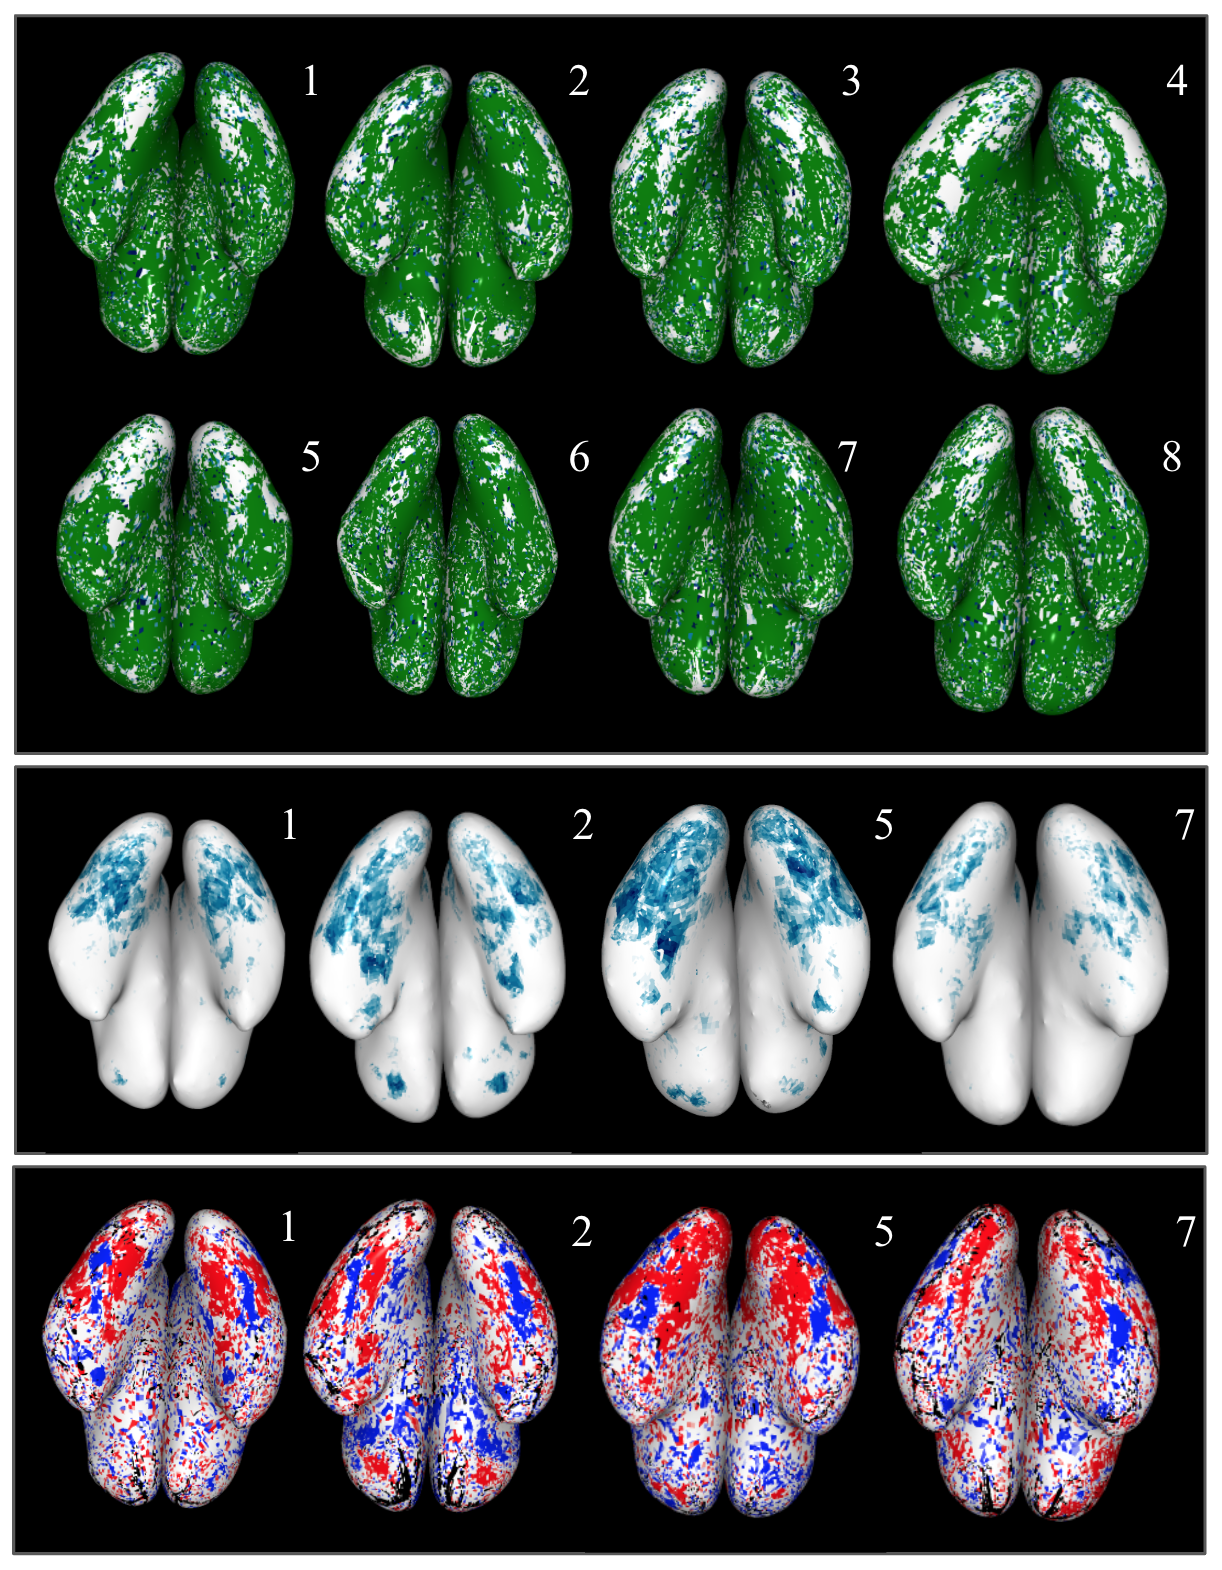
\includegraphics[scale=0.55]{fig2.png}
        \caption{This figure shows voxels that are determined to be food-related based off of two differing methods. The top image shows significant voxels (white) from a 1-sided t-test comparing food weights from a trained OLS model against all other non-food object weights. The middle image shows classification accuracy for voxel-wise searchlight decoding, with darker blue voxels signifying higher accuracy. The bottom image shows significant voxels from a 1-sided t-test comparing food weights against face weights (red) as well as the results for a 1-sided t test comparing face weights against food weights (blue). It is notable here to compare significant 'food' voxels to 'face' voxels because the of the high number of face images in our dataset, as well as the robust reliability of the FFA. The food-related regions resulting from both methods overall align with each other, suggesting that these regions are reliably more responsive to food stimuli than other categories. } \label{fig1}
    \end{figure}

\section{Decoding Models}
The high-accuracy voxels from the searchlight decoding model overall align spatially with the significant voxels from the encoding model, as is clear in Figure 2. We note that high-accuracy voxels do not necessarily correspond to food-selective regions, but rather to any region which helps identify whether or not the given stimuli contains food. So, high-accuracy voxels can signify both a food-selective region and an anti-food selective region that especially helps determine that the stimuli is not food-related. 
Running a voxel-wise searchlight classification allows an investigation into food-reactive voxels from a different perspective from the previously mentioned encoding model. The inclusion of the previously identified food regions in the high-accuracy searchlight voxels further confirms our proposed food regions. Similar regions as those found in the encoding model are observed to be highly correlated with the stimuli food classification accuracy. \\

Both the encoding and decoding models confirm that these regions seem to be consistently more reactive to food than other categories. However, these models provide little insight into the more fine grained semantic and spatial structure of the responses within this food region. To discover these intra-region patterns, we run a principled component analysis (PCA) on the selected visual cortex regions and investigate the relevant contributing images. 

\section{Semantic Regions Axes}
Running PCA on the hypothesized food region leads to a further spatial breakdown of various 'food' areas, as is shown in Figure 3. These breakdowns are able to account for a significant portion of the variance of this region's responses. Each of the uncovered components' axes seems to correspond with a general semantic pattern of image content. To achieve these components, we perform PCA on the matrix of the proposed food regions' voxels by the 108 food-related images from our dataset. The top components explain 34.31, 12.68, and 11.16 percent of the variability, respectively. These components, each appearing to correspond to varying semantic characteristics, have unique contributions to this region's activity. These results demonstrate that explaining the variance of this proposed food region can be done via components with unique correspondences to semantic categories.
    \begin{figure}
        \centering
        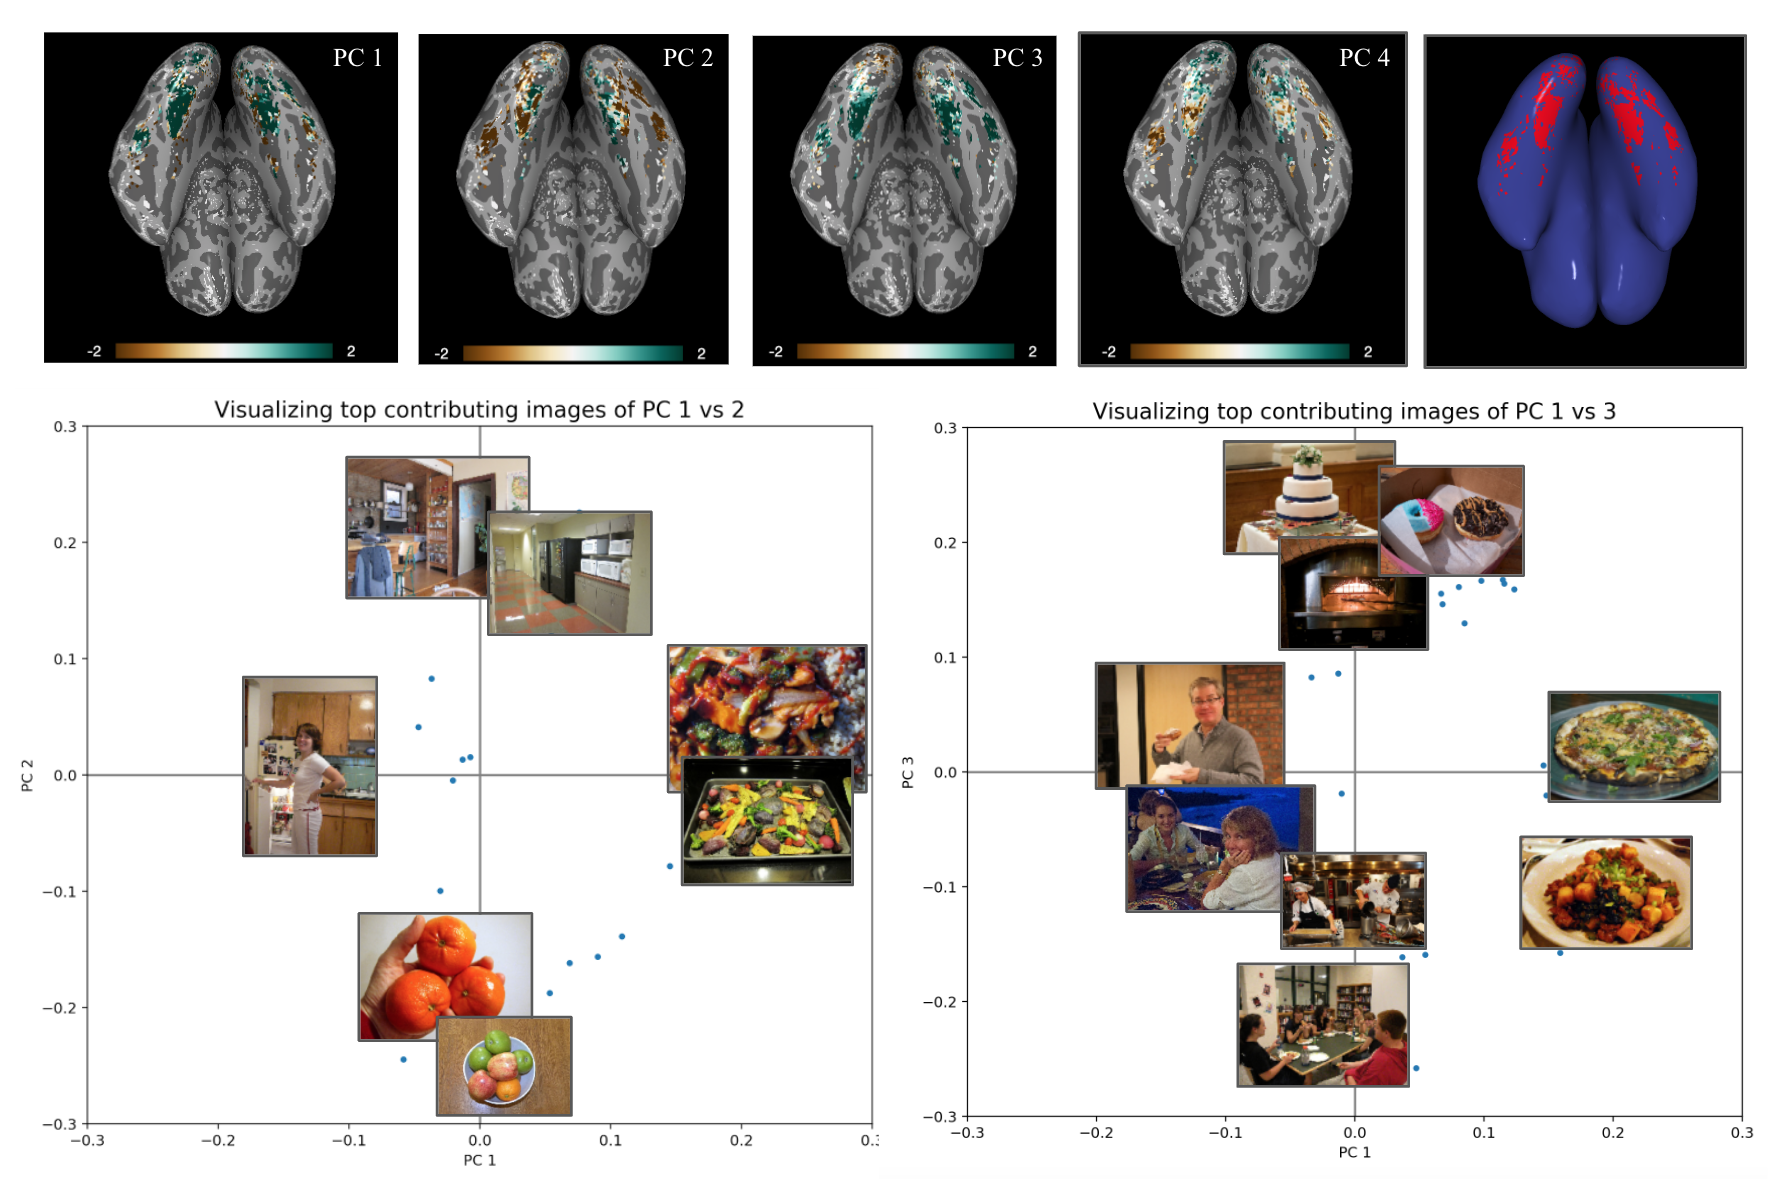
\includegraphics[scale=0.45]{fig3.png}
        \caption{Applying PCA on the proposed food region's responses provides more insight into the structure of these responses. Above, we can see the different regions corresponding to different components, as well as the top images for each component. The top images display each components projection onto the brain, demonstrating the generally positively (green) and negatively (brown) contributing voxels. On the top right, we see in red the region that we have identified as the relevant food region, generated based off of the intersection of the food vs face encoding model test and manually identified visual cortex regions. In the graphs, we see stimuli that most contribute to various components, as well as their placement. We see that each component overall highlights different semantic characteristics of the visual stimuli. The first component appears captures the surface area of food in the image, the second distinguishes places, and the third seems to capture a combination of spatial frequency and people. These semantic categories are able to explain a large component of the variance resulting from these food regions.} \label{fig1}
    \end{figure}

\section{Generalizing Across all Stimuli}
We further consider voxel responses to food by inspecting how voxels react to specific food categories from images not yet inspected when proposing the food region. In order to use images not yet inspected, we consider the remaining images that were not viewed by all 8 subjects. We run a voxel-wise ridge regression on the provided COCO labels on these images to predict voxel activity. Then, we visualize the resulting weights per label on each voxel, as shown in Figure 4. In order to observe the which voxels' prediction accuracies benefit most from the addition of food labels, we perform the ridge regression on all labels, as well as all but food labels. We then compare the $R^{2}$ values voxel-wise. We observe one general activation pattern by the food-related labels. This pattern corresponds strongly with our previously proposed food region, and aligns with the subset of voxels whos' prediction performance improves due to the addition of food labels. This improvement suggests that these voxels are more responsive to food than other cortical areas. Activations across the food labels are extremely consistent.The responses re-emphasize our identification of a food-selective region. 
    \begin{figure}
        \centering
        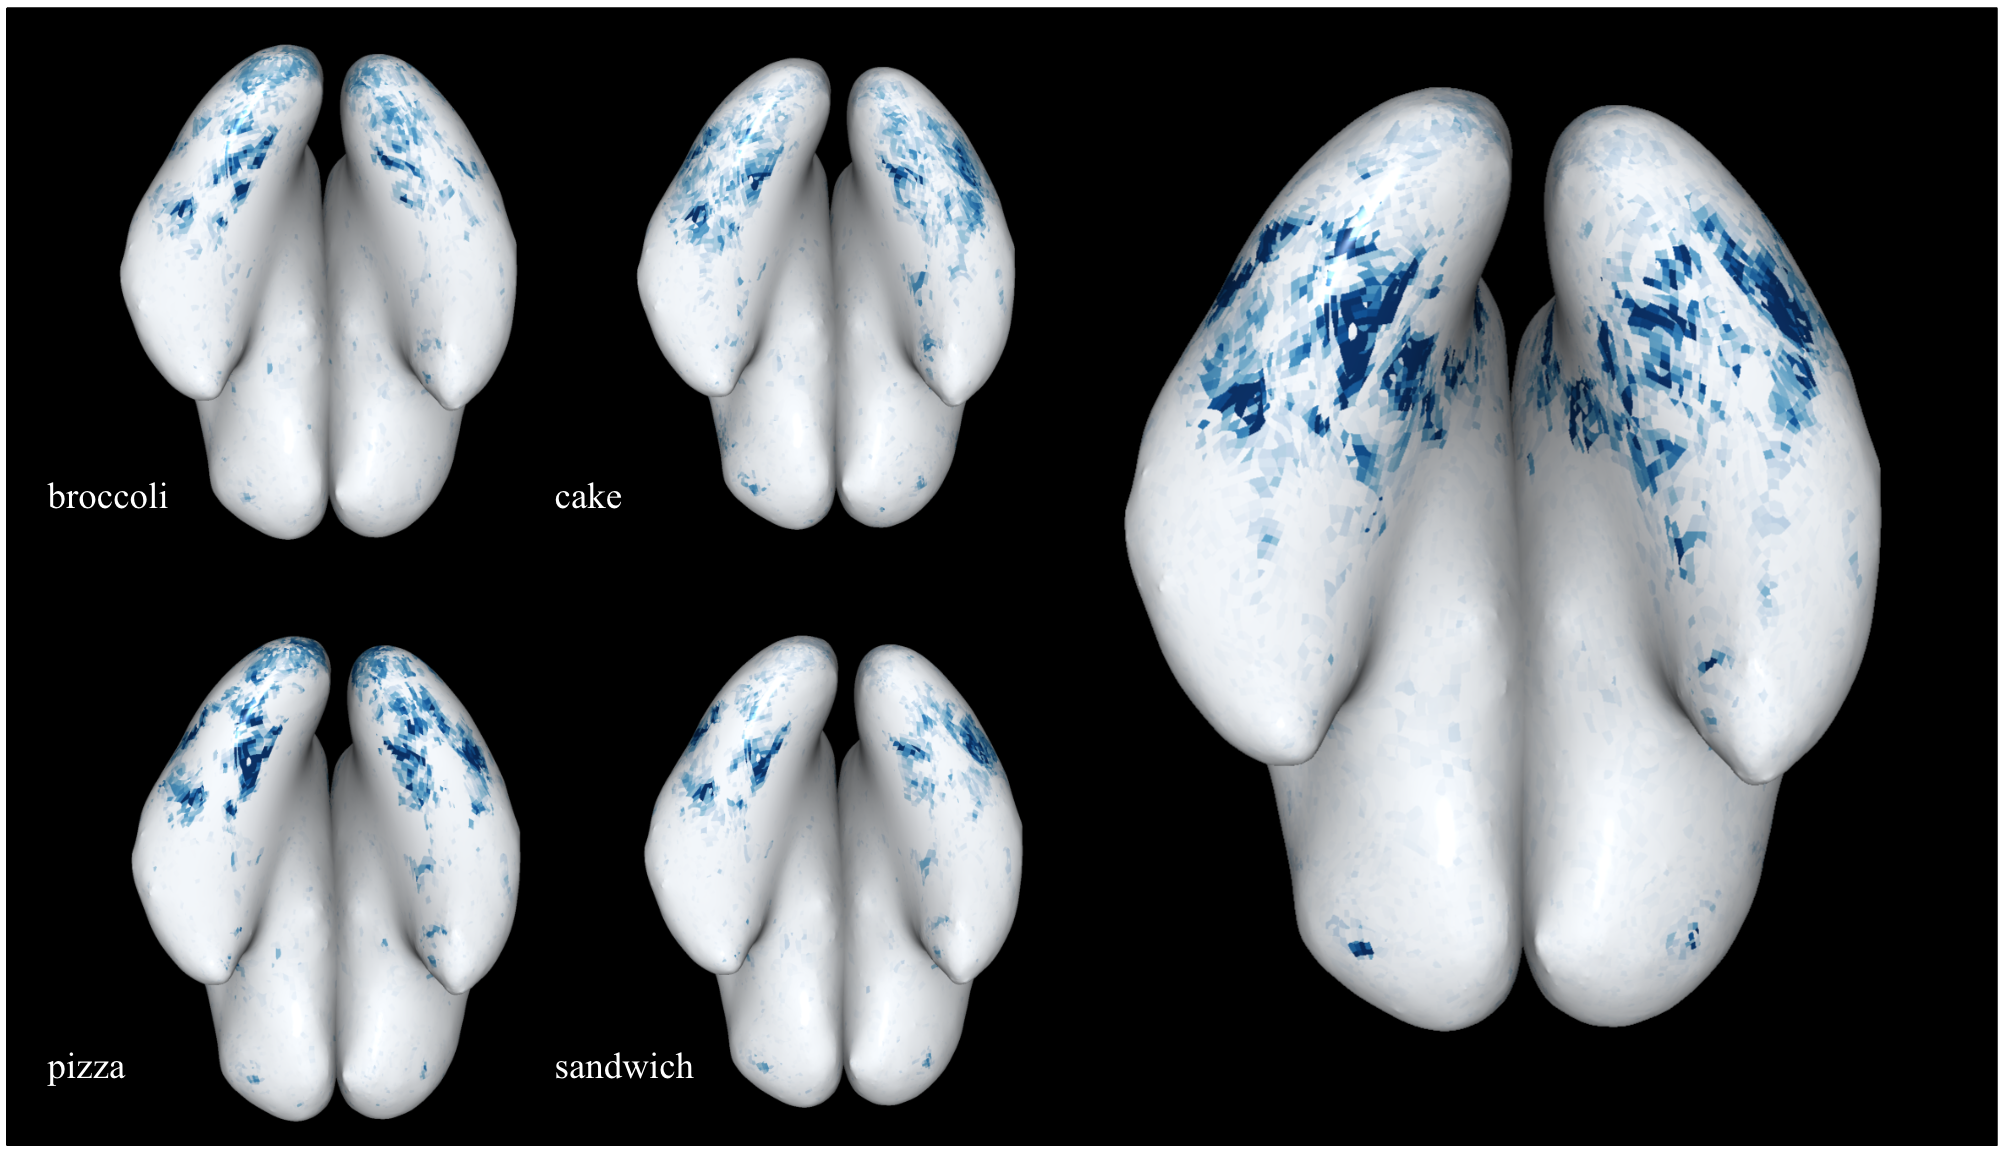
\includegraphics[scale=0.45]{fig4.png}
            \caption{Analysis on predicting voxel activity from unseen images points to the same food-selective regions as previously proposed. We observe 4 COCO label weights corresponding to each voxel following a voxel-wise ridge regression on COCO labels (left) We also observe the voxel-wise improved $R^{2}$ values from including food labels when predicting voxel activity (right). Both the weights corresponding to individual food labels as well as the overall impact of the aggregate food labels highlight our proposed food regions. These results also point to the conclusion that this region is food selective.} \label{fig1}
    \end{figure}
 
\section{Voxel Embedding Clusters vs Deep Learning Embedding Clusters}    
To confirm that our proposed region does in fact have this unique food selection, we test whether our proposed food region responds to new food-related images significantly differently from new non-food related images. In this test, our new subset of images also includes an even split of non-food and food images from images that were not used to determine the originally proposed food region. Using the previously proposed mask of voxels identified as food-selective, we create a subset of corresponding voxel activity for each image. We then use the K-means algorithm to cluster the voxel data corresponding to these images to reveal patterns of reactivity in this region. 2 clusters emerge, each containing voxel activity corresponding to an image. We now consider the images corresponding to this voxel activity, and thus the 2 clusters of images. We notice that 1011 of the 1638 food images gather in one cluster, and observe the images with the highest voxel activity in each cluster (Figure 5). The top images in each cluster have significant semantic differences, with one cluster clearly corresponding highly with food. These top cluster images further confirm our proposal of this region as selective to food. 
    \begin{figure}
        \centering
        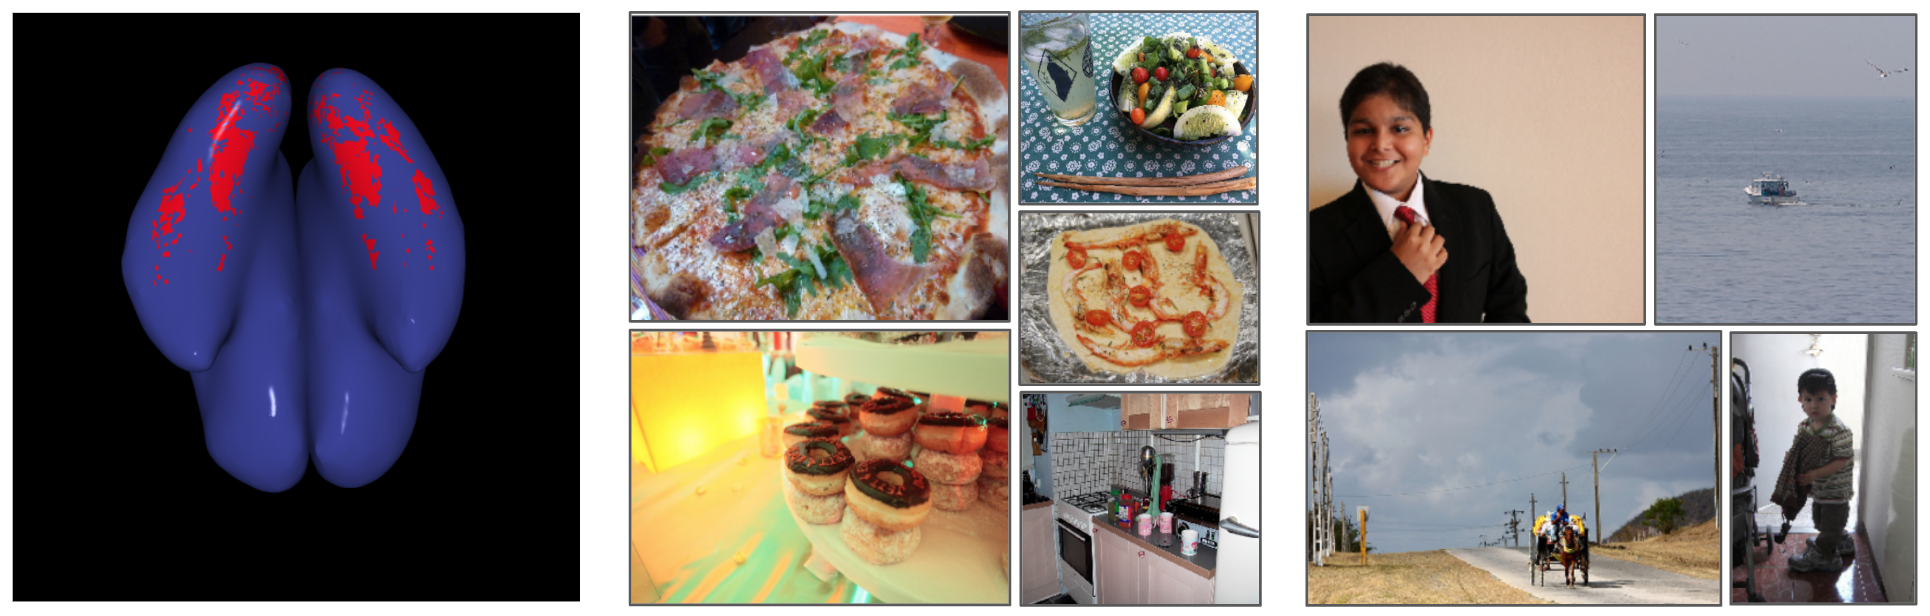
\includegraphics[scale=0.47]{fig5.png}
            \caption{We observe the highest voxel-activity inducing images in each cluster. This helps us identify how our proposed food region reacts to different images. On the left we see in red the voxels identified as the proposed food region, and thus used here to cluster the images. In the middle we see top images corresponding to our first cluster, and on the right we see the top images corresponding to the second cluster. We clearly this region reacts differently to food than to other images. } \label{fig1}
    \end{figure}

We use voxel responses to further cluster food images and observe the resulting clusters. Especially when considering the visual cortex, it is important to isolate causes for variations in brain responses from solely image feature variation. To help understand if variations in food responses are due to visual characteristics, we use CLIP and ResNet to cluster food-related images and observe resulting patterns. We then observe whether these patterns are consistent with the clusters emerging from voxel-based image clustering. CLIP considers both visual and semantic features when training, while ResNet only considers visual features. In both outputs, we notice semantic clusters that do not have clear correspondence with our resulting food clusters (Figure 6), suggesting likely top down processing that goes further than raw visual features. 

    \begin{figure}
        \centering
        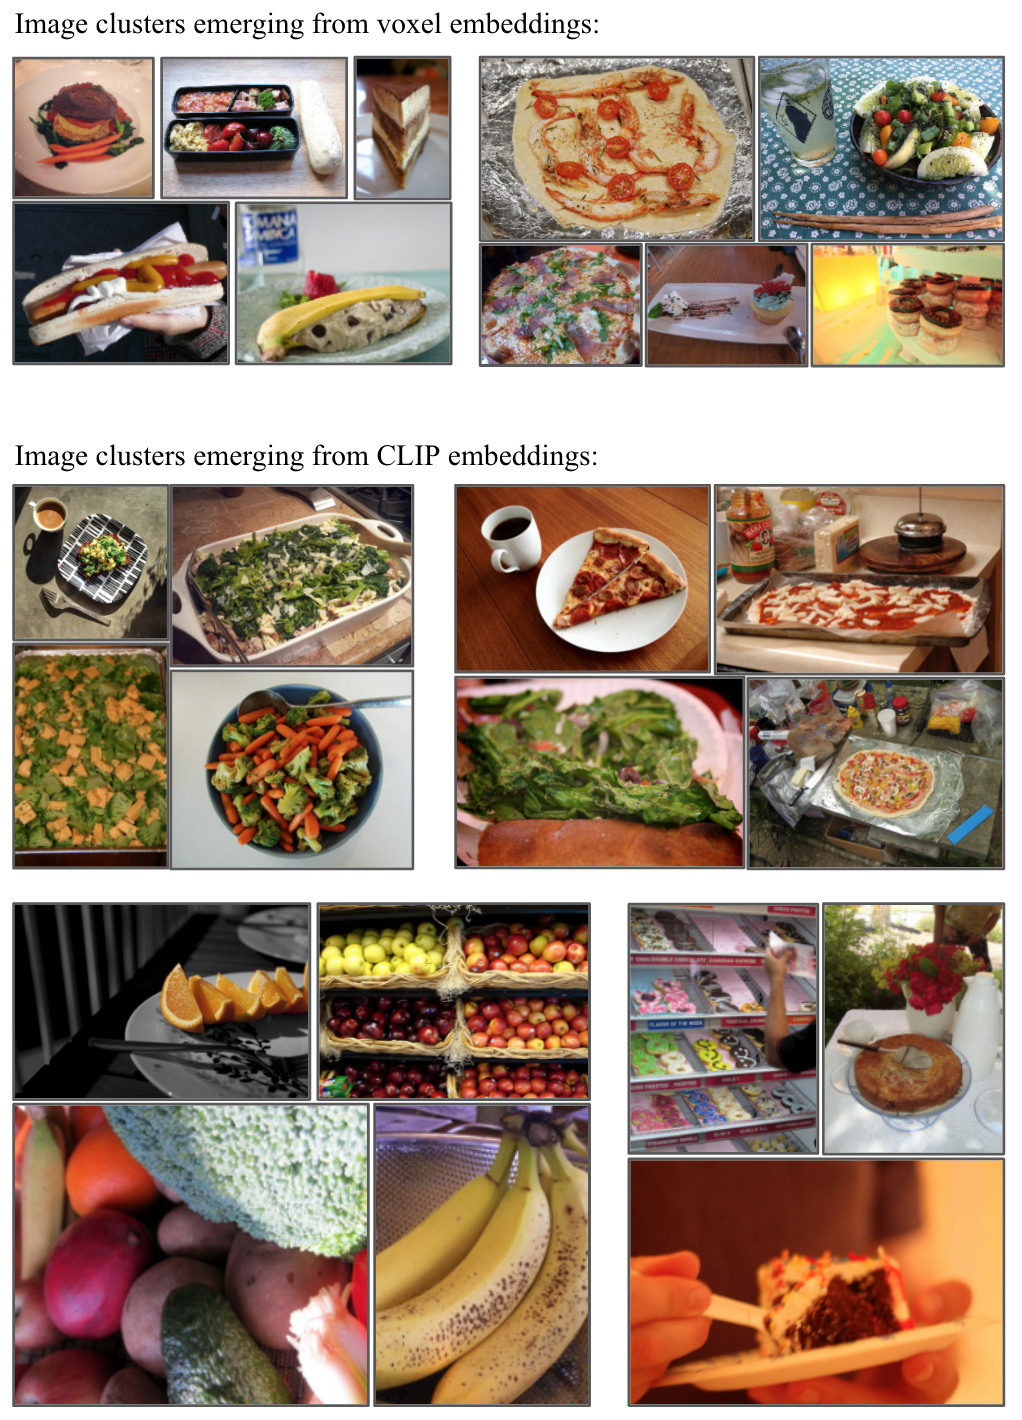
\includegraphics[scale=0.55]{fig6.png}
            \caption{We observe image clusters based on voxel-response embeddings (top). We then compare this to image clusters based on CLIP embeddings (bottom). Two clusters emerge from voxel-response embeddings, while 4 main clusters emerge from CLIP. The two clustering patterns show little to no correlation with each other, demonstrating that this proposed food region involves more complex, top down processing rather than solely low level or semantic features. } \label{fig1}
    \end{figure}


\end{document}